%	PACKAGES AND THEMES
%----------------------------------------------------------------------------------------
\documentclass[xcolor=dvipsnames,t,9pt]{beamer}
%\documentclass[aspectratio=169,xcolor=dvipsnames,t,9pt]{beamer} %for 16:9 ratio slide
\usetheme{Symply}

\usepackage{hyperref}
\usepackage{graphicx} 
\usepackage{booktabs} 
\usepackage{multirow}
\urlstyle{same}
\usepackage{appendixnumberbeamer}

\setbeamertemplate{bibliography item}{[\arabic{enumiv}]}

%----------------------------------------------------------------------------------------
%	TITLE PAGE FOR RESEARCH PRESENTATION
%----------------------------------------------------------------------------------------

\title{Fairness-Aware Optimal Market Participation of \\Aggregated Distributed Energy Resources}
\subtitle{Term Project}
\author[장서현 $|$]{\textbf{장서현 (jangseohyun@yonsei.ac.kr)}\inst{1}} % set short author for author name in footline 
\institute[연세대학교 산업공학과] 
{
  \inst{1}\textbf{SY}stems \textbf{M}odeling and \textbf{P}rogramming \textbf{L}ab \\Department of Industrial Engineering, \textbf{Y}onsei University - \textbf{SYMPLY} \\
  (\url{https://symply.yonsei.ac.kr/})
}  % set short institute for department and institute in footline 
\date[IIE7585 확률적계획법 $|$]
{
    IIE7585 확률적계획법\\\bigskip
    \centerline{\includegraphics[width=0.4\textwidth]{logo_text.png}}
} % set shortdate for conference title in footline


%----------------------------------------------------------------------------------------
%   기존 폰트 설정 부분
%----------------------------------------------------------------------------------------
% \usepackage[T1]{fontenc}
% \usepackage[usefilenames,DefaultFeatures={Ligatures=Common}]{plex-otf} %
% \renewcommand*\familydefault{\sfdefault} %% Only if the base font of the document is to be sans serif

% \usepackage[unfonts]{kotex}
% \xetexkofontregime{latin}[puncts=prevfont, colons=prevfont, cjksymbols=hangul]
% \setmainhangulfont{NanumSquare}
% \setsanshangulfont{NanumSquare}
% \setmonohangulfont{NanumSquare}

%NanumGothic, NanumSquare, Noto Sans CJK KR

%----------------------------------------------------------------------------------------
%   다른 방식의 폰트 설정 부분
%----------------------------------------------------------------------------------------
\usepackage{kotex}
\usepackage{fontspec}
\setsansfont{IBMPlexSans}[
    Path=./IBMPlexSans/,
    Extension = .ttf,
    UprightFont=*-Light,
    BoldFont=*-Medium,
    ItalicFont=*-LightItalic,
    BoldItalicFont=*-MediumItalic,
    ]
% Light and Medium from IBMPlexSansKR for both English and Korean
% LightItalic and MediumIntalic from IBMPlexSans for only English

% \usepackage{kotex}
% \usepackage{fontspec}
% \setsansfont{NotoSansKR}[
%     Path=./NotoSansKR/,
%     Extension = .ttf,
%     UprightFont=*-Light,
%     BoldFont=*-Light,
%     % ItalicFont=*-Italic,
%     % BoldItalicFont=*-BoldItalic,
%     ]



%----------------------------------------------------------------------------------------
%	PRESENTATION SLIDES
%----------------------------------------------------------------------------------------

\begin{document}

{
\setbeamertemplate{headline}{} % no headline on title page
\setbeamertemplate{footline}{} % no footline on title page
\begin{frame}[noframenumbering] % no page count on title page
    % Print the title page as the first slide
    \titlepage
\end{frame}
}

% {
% \setbeamertemplate{headline}{} % no headline on title page
% \setbeamertemplate{footline}{} % no footline on title page
\begin{frame}{목차} % no page count on title page
    % Throughout your presentation, if you choose to use \section{} and \subsection{} commands, these will automatically be printed on this slide as an overview of your presentation
    \tableofcontents
\end{frame}
% }

%------------------------------------------------
\section[문제 배경]{문제 배경}
%------------------------------------------------

\begin{frame}{분산에너지원 (Distributed Energy Resources, DER)}
    \textbf{에너지를 사용하는 공간ㆍ지역 또는 인근지역에서 공급하거나 생산하는 에너지로, 일정 규모 이하의 소규모 에너지 \footnotemark[1]}
    \begin{itemize}
        \item 태양광(PV) 및 풍력 터빈(WT) 발전 장치, 에너지 저장 시스템(ESS), 전기 자동차(EV) 충전기, 마이크로그리드 등을 포함
        \item 소규모 발전의 형태에 적합한 탄소중립적인 에너지를 중심으로 생산
    \end{itemize}

    \begin{block}{}
        $\Rightarrow$ 불안정한 대규모 중앙집중식 송전 및 발전에서 벗어나, 수요지 인근에서 환경친화적이고 독립적인 에너지의 생산과 소비 가능
    \end{block}

    \footnotetext[1]{대한민국 정부, 분산에너지 활성화 특별법 (2023), \url{https://www.law.go.kr/법령/분산에너지활성화특별법}}

\end{frame}

%------------------------------------------------

\begin{frame}{전력시장 (Wholesale Electricity Market)}
    \small
    \setlength{\columnsep}{0pt}
    \begin{columns}
        \column{0.5\textwidth}
        \raggedright
        \textbf{하루전시장 Day-ahead Commitment Market} \vspace{0.2em}
        \begin{itemize}
            \item 하루 전에 예측된 수요와 공급 기반으로 다음날 시간별 가격이 결정됨
            \item 공시된 가격에 따라 일정량의 전력 공급/소비를 \textbf{하루 전에 계약} (commitment)
            \item 계약 불이행 시 페널티 발생
        \end{itemize}
        \column{0.45\textwidth}
        \raggedright
        \textbf{실시간시장 Real-time Balancing Market} \vspace{0.2em}
        \begin{itemize}
            \item 실시간 수요와 공급 차이를 조정하는 시장
            \item 5분에서 20분 간격으로 \textbf{실시간 가격 책정 및 수급 조정}
            \item Day-ahead 시장가보다 평균적으로 낮으며, 가격 변동성이 큼
        \end{itemize}
    \end{columns}

    \vspace{7pt}

    \begin{figure}[htb!]
        \centering
        \begin{minipage}[t]{0.48\linewidth} % 동일한 너비 지정
            \centering
            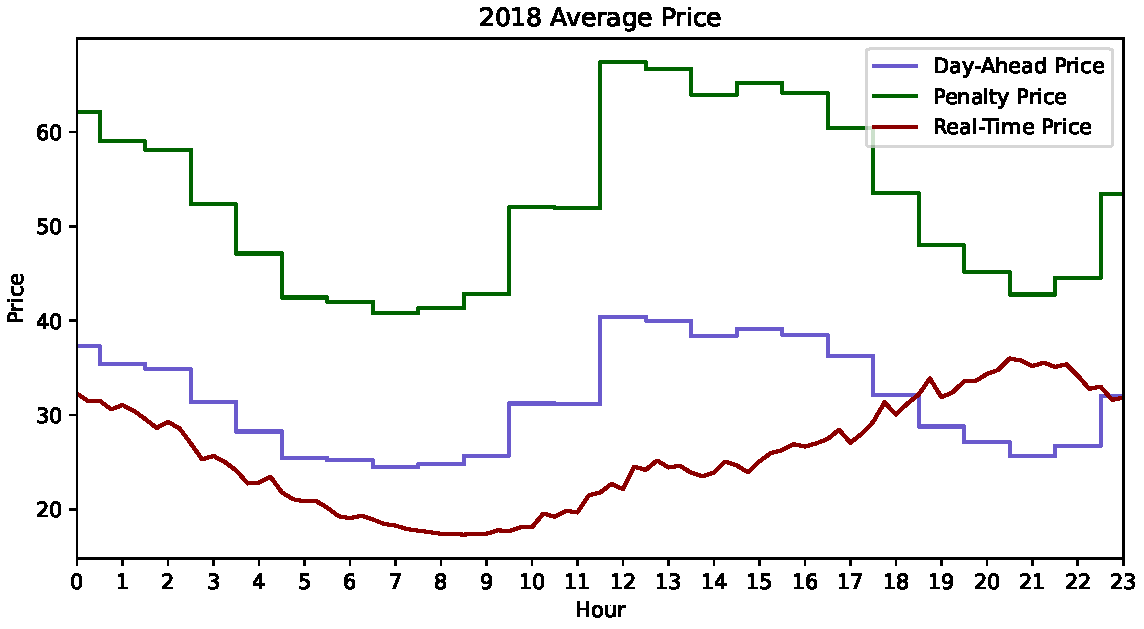
\includegraphics[width=\linewidth]{fig_avgprice.pdf}
            \caption{Annual Average Electricity Price \footnotemark[2]}
            \label{fig:avgprice}
        \end{minipage}
        \begin{minipage}[t]{0.48\linewidth} % 동일한 너비 지정
            \centering
            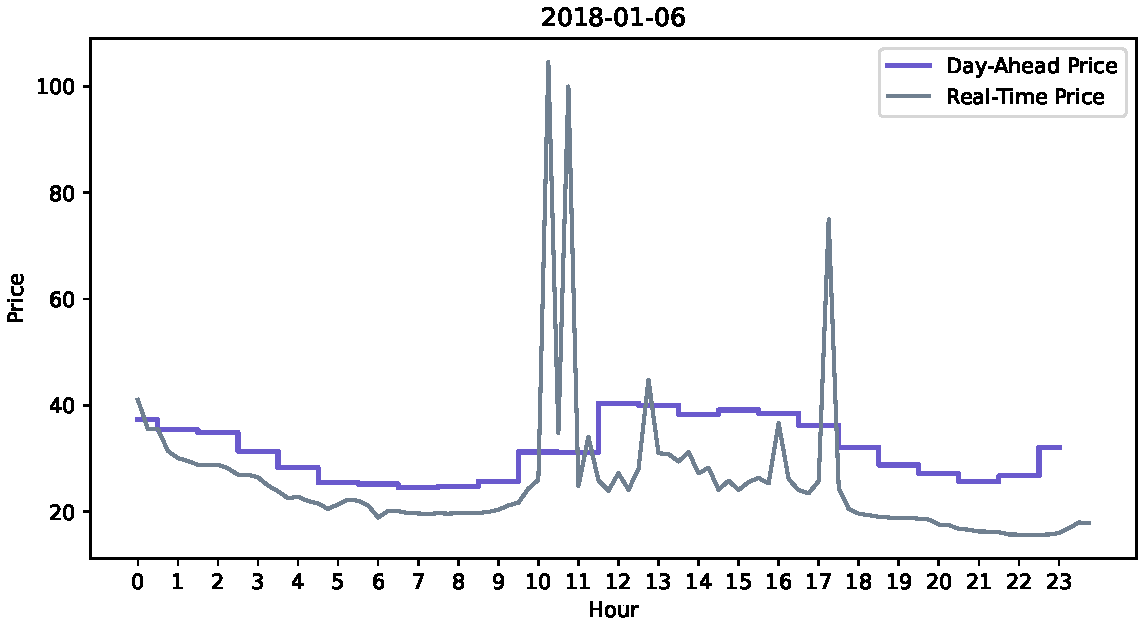
\includegraphics[width=\linewidth]{fig_price.pdf}
            \caption{Variability in Real-Time Price \footnotemark[2]}
            \label{fig:price}
        \end{minipage}
        \hfill
    \end{figure}
    \footnotetext[2]{Pecan Street Inc., Pecan Street Dataport, 2018, \url{https://www.pecanstreet.org/dataport}}
\end{frame}

%------------------------------------------------

\begin{frame}{분산에너지원의 통합 (Aggregation)}
    \textbf{여러 개별 분산에너지원들을 하나의 포토폴리오(Aggregated Distributed Energy Resources, ADER)로 통합하는 과정으로, 가상 발전소나 에너지 관리 시스템 등을 통해 구현}
    \begin{block}{Aggregation이 필요한 이유}
        \textcircled{\small{1}} 재생에너지 발전량의 불확실성과 \textcircled{\small{2}} non-dispatchable한 출력 특성으로 인해,\\ 안정적인 day-ahead commitment를 하기 어렵고 그에 따라 페널티가 부과될 위험이 높음
    \end{block}

    \vspace{0.7em}

    \textbf{개별 DER들은 Aggregation을 통해}
    \begin{itemize}
        \item 서로의 발전잉여량과 계약미충족량을 상쇄시킴으로써 페널티 리스크 완화
        \item 하나의 포토폴리오로서 최적화된 day-ahead commitment와 real-time trading 수행
    \end{itemize}
    \begin{figure}[h]
        \centering
        \begin{minipage}{0.325\textwidth}
            \centering
            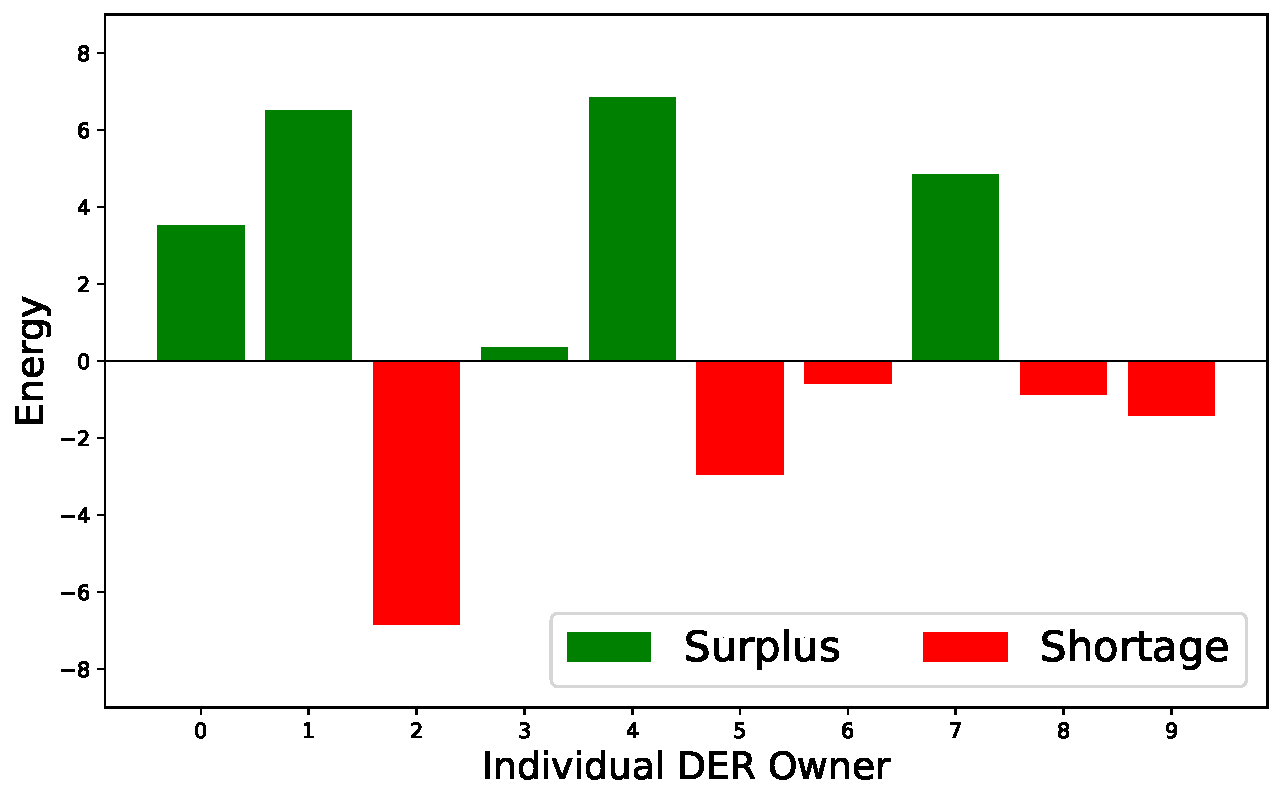
\includegraphics[width=\linewidth]{fig_pool1.pdf}
            \caption{Pre-Pooling}
        \end{minipage}
        \begin{minipage}{0.325\textwidth}
            \centering
            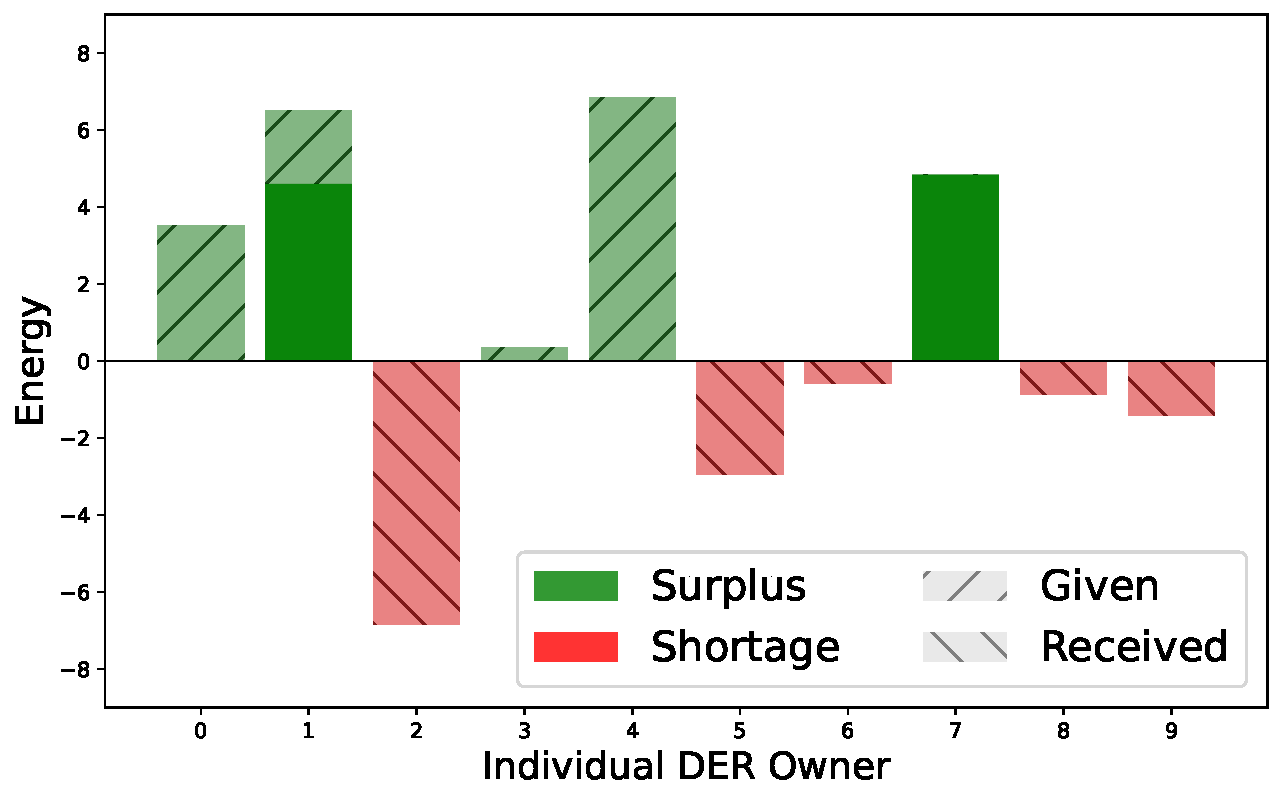
\includegraphics[width=\linewidth]{fig_pool2.pdf}
            \caption{Pooling Process}
        \end{minipage}
        \begin{minipage}{0.325\textwidth}
            \centering
            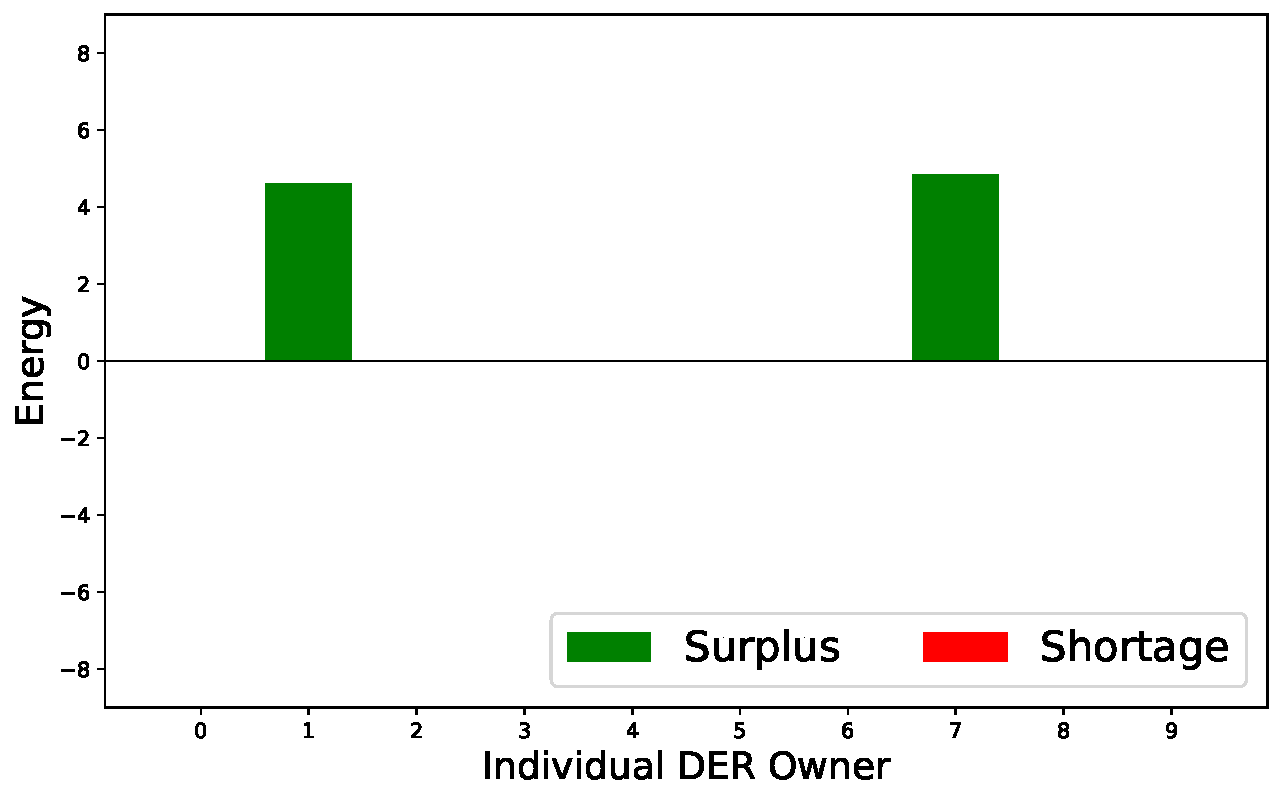
\includegraphics[width=\linewidth]{fig_pool3.pdf}
            \caption{Post-Pooling}
        \end{minipage}
    \end{figure}

\end{frame}

%------------------------------------------------

\begin{frame}{공정성에 대한 고려}
    발전량 패턴이 다양한 참여자가 많을수록 Aggregation의 효과가 커짐
    \vspace{-1em}
    \begin{table}[]
        \caption{Aggregation 참여자 수에 따른 수익률 차이}
        \footnotesize
        \begin{tabular}{lccc}
            \hline
            참여자 수            & 5             & 10             & 15             \\ \hline
            개별 참여 수익의 합 (\$) & 4531.18       & 8508.44        & 10986.16       \\
            통합 참여 수익 (\$)    & 4885.48       & 9422.01        & 12334..29      \\ \hline
            차이 (\%)          & \textbf{7.81} & \textbf{10.74} & \textbf{12.27} \\ \hline
        \end{tabular}
    \end{table}
    \vspace{-0.5em}
    \begin{alertblock}{}
        포트폴리오 내에서 개별 DER의 에너지가 \textbf{불공정하게 활용}된다면, Aggregation에 참여할 유인이 감소하고 \textbf{참여자의 이탈}이 발생할 수 있음
        \begin{itemize}
            \item 페널티 발생 위험 증가
            \item 집합체 수준의 기대 수익 감소
            \item 개별적으로 정산받을 수 있는 양 감소
        \end{itemize}
        $\Rightarrow$ 포토폴리오 내의 개별 DER들 사이 공정성이 고려되어야 함
    \end{alertblock}

    \underline{본 프로젝트에서의 공정성 정의:}
    \begin{itemize}
        \item \textbf{기여도 기반}: 포토폴리오의 페널티 방지를 위해 각 참여자가 기여한 정도가 유사해야 함
        \item 기여도는 \textbf{기여 에너지양과 해당 시간의 시장가격}을 함께 고려하여 측정
    \end{itemize}

\end{frame}

%------------------------------------------------
\section[문제 정의]{문제 정의}
%------------------------------------------------

\begin{frame}{문제 정의}
    ADER의 시장 참여 전략을 수립하기 위해, 각 시간대별로 다음과 같은 결정들이 필요함
    \begin{itemize}
        \item \textbf{하루전시장}에 제출할 \textbf{Commitment 양}
        \item \textbf{실시간시장}에서의 \textbf{판매량}, Commitment \textbf{미충족량}
        \item \textbf{에너지 저장 장치}의 \textbf{충$\cdot$방전량}
        \item \textbf{Aggregation의 페널티 방지}를 위한 기여량
    \end{itemize}

    \begin{block}{}
        위 결정 변수들은 \textbf{포토폴리오의 총 이익을 최대화}하는 방향으로 결정되어야 하며, \textbf{포트폴리오 내 개별 DER 참여자의 에너지 활용 방식} 또한 함께 결정되어야 함
    \end{block}

    \vspace{-1em}

    \begin{table}[]
        \caption{의사결정 시점에 따른 결정변수 구조}
        \small
        \renewcommand{\arraystretch}{1.3}
        \begin{tabular}{cccc}
            \hline
            \multicolumn{1}{l}{}                                        & \multicolumn{1}{l|}{}                            & Agg.                             & Ind. ($i$)     \\ \hline
            \multicolumn{1}{c|}{\textbf{Here-and-now}}                  & \multicolumn{1}{c|}{하루전시장에서의 commitment 결정}      & $\alpha \left(= \sum x_i\right)$ & $x_i$          \\ \hline
            \multicolumn{4}{c}{\textbf{불확실성 실현} (실시간 가격, 재생에너지 발전량)}                                                                                                           \\ \hline
            \multicolumn{1}{c|}{\multirow{3}{*}{\textbf{Wait-and-see}}} & \multicolumn{1}{c|}{실시간시장에서의 판매량 / 계약미충족량}       & $\beta \left(= \sum y_i \right)$ & $y_i$          \\ \cline{2-4}
            \multicolumn{1}{c|}{}                                       & \multicolumn{1}{c|}{에너지 저장 장치의 충방전량}             &                                  & $z_i^C, z_i^D$
            \\ \cline{2-4}
            \multicolumn{1}{c|}{}                                       & \multicolumn{1}{c|}{Aggregation의 페널티 방지를 위한 기여량} &                                  & $d_i$
            \\ \hline
        \end{tabular}
    \end{table}

\end{frame}

%------------------------------------------------

\begin{frame}{방법론 소개}
    \begin{block}{Risk-Averse Two-stage Stochastic Optimization Model}
        \textbf{Objective Function} \\
        \begin{itemize}
            \item 수익 최대화 (하루전시장 수익 + 실시간시장 판매량 - 하루전시장 미충족 페널티)
            \item DER 간 기여도 편차를 리스크로 간주하여, 평균보다 적거나 많은 기여도 모두에 대해 페널티 부여
        \end{itemize}
        \textbf{First-Stage}: 불확실성 실현 \underline{이전}
        \begin{itemize}
            \item 하루전시장에 제출할 Commitment 양 $\left( \alpha, x_i \right)$
        \end{itemize}
        \textbf{Second-Stage}: 불확실성 실현 \underline{이후}
        \begin{itemize}
            \item 실시간시장에서의 판매량 / 계약미충족량 $\left( \beta(\xi), y_i(\xi)\right)$
            \item 에너지 저장 장치의 충$\cdot$방전량 $\left(z_i^C(\xi), z_i^D(\xi) \right)$
            \item Aggregation의 페널티 방지를 위한 기여량 $\left( d_i(\xi) \right)$
        \end{itemize}
    \end{block}
    \vspace{0.5em}
    \textbf{Sampling-based Approach}를 활용하여 실시간 시장 가격이나 발전량의 불확실성 고려 \\
    $\rightarrow$ 각 시나리오들은 historical data를 바탕으로 구성되며, second-stage decision
    variable들과 stochastic parameter들은 scenario-dependent하게 $\xi_s$ 로 재정의됨

\end{frame}

%------------------------------------------------

\begin{frame}{공정성 기반 위험 측정 (Fairness-Aware Risk Factor)}
    각 DER \(i\)의 $T$시간 동안의 시나리오$(\xi_s)$별 총 기여도(금액):
    \[
        \Lambda_{i}(\xi_s) = \sum_{t \in T} d_{it}(\xi_s) \cdot (P^{PN}_t - P^{RT}_{t}(\xi_s))
    \]
    \vspace{-1em}
    \begin{itemize}
        \item 각 DER이 실시간 시장에서 판매하여 얻을 수 있던 수익 중 일부($d \cdot P^{RT}$)를, 포트폴리오 전체의 페널티 회피($d \cdot P^{PN}$)를 위해 양보했다고 해석
        \item 개인의 기회비용으로서 정의되는 marginal contribution을 기여도로 간주
    \end{itemize}
    \vspace{-0.5em}
    \begin{alertblock}{Central Deviation 활용}
        포트폴리오의 공정성을 확보하기 위해, 각 DER의 기여도 금액이 평균에서 벗어나는 경우에 대해 리스크로 간주하는 \textbf{양방향 절대편차 기반 측도} 도입
        \[
            \phi_{\text{CDEV}}(\Lambda_i) := \mathbb{E}_s \big[ \left| \Lambda_i(\xi_s) - \mathbb{E}_i[\Lambda_i(\xi_s)] \right| \big]
        \]
        \vspace{-1.5em}
        \begin{itemize}
            \item 과도하게 기여하거나 충분히 기여하지 않은 DER 모두를 공정성 위반으로 간주
            \item 공정성은 전체 시나리오에서의 기여 편차를 지속적으로 관리해야 실질적으로 보장되므로, tail risk만 반영하는 quantile risk measure보다 deviation-based 측도가 더 적합하다고 판단
        \end{itemize}
    \end{alertblock}

\end{frame}

%------------------------------------------------
\section[수리 모델]{수리 모델} %[Section Short Name] will be displayed in headline
%------------------------------------------------

\begin{frame}{결정변수 및 파라미터 정의}
    \small
    \begin{minipage}{0.47\textwidth}
        \textbf{인덱스}
        \begin{itemize}
            \item $i \in I$:
            \item $t \in T$:
            \item $s \in S$:
        \end{itemize}
        \textbf{파라미터}
        \begin{itemize}
            \item $P_t^{DA}$:
            \item $P_t^{RT}(\xi)$:
            \item $P_t^{PN}$:
            \item $R_{it}(\xi)$:
            \item $K_i$:
            \item $M_1, M_2$:
            \item $\lambda$
        \end{itemize}
    \end{minipage}
    \begin{minipage}{0.47\textwidth}
        \textbf{결정변수}
        \begin{itemize}
            \item $x_{it}$
            \item $y_{it}^{+}(\xi)$
            \item $y_{it}^{-}(\xi)$
            \item $z_{it}(\xi)$
            \item $z^C_{it}(\xi), z^D_{it}(\xi)$
            \item $d_{ijt}(\xi)$
            \item $e^+_{it}(\xi)$
            \item $e^-_{it}(\xi)$
            \item $\Lambda_i(\xi)$
            \item $\Delta_i(\xi)$
            \item $\phi^1_{it}(\xi_s), \phi^2_{it}(\xi_s), \phi^3_{it}(\xi_s), \phi^4_{t}(\xi_s) \in \{0,1\} $    
        \end{itemize}
    \end{minipage}
\end{frame}

%------------------------------------------------

\begin{frame}{수리 모델 (1)}

    목적함수 제약식일부 설명
\end{frame}

%------------------------------------------------

\begin{frame}{수리 모델 (2)}

    제약식 일부 설명
\end{frame}

%------------------------------------------------

\begin{frame}{수리 모델: Risk-Neutral 모델}
    \vspace{-1em}
    \begin{subequations}
        \footnotesize
        \begin{align}
            \text{max} \quad  & \sum_{t\in T}\left(P_t^{DA} \sum_{i \in I}x_{it} + \mathbb{E}\left[P_t^{RT}(\xi_s)\sum_{i \in I}e^+_{it}(\xi_s) - P_t^{PN}\sum_{i \in I}e^-_{it}(\xi_s)\right]\right) &                 \\
            \text{s.t.} \quad & R_{it}(\xi_s) - x_{it} = y_{it}^{+}(\xi_s) - y_{it}^{-}(\xi_s) + z^C_{it}(\xi_s) - z^D_{it}(\xi_s)                                                                    & \forall i, t, s \\
                              & R_{it}(\xi_s) \geq y^+_{it}(\xi_s)                                                                                                                                    & \forall i, t, s \\
                              & z_{i,t+1}(\xi_s) = z_{it}(\xi_s) + z^C_{it}(\xi_s) - z^D_{it}(\xi_s)                                                                                                  & \forall i, t, s \\
                              & z^D_{it}(\xi_s) \le z_{it}(\xi_s), \quad z^C_{it}(\xi_s) \le K_i-z_{it}(\xi_s), \quad 0 \leq z_{it}(\xi_s) \leq K_i                                                   & \forall i, t, s \\
                              & e^+_{it}(\xi_s) = y^+_{it}(\xi_s) - \sum_{j \in I}d_{ijt}(\xi_s), \quad e^-_{it}(\xi_s) = y^-_{it}(\xi_s) - \sum_{j \in I}d_{jit}(\xi_s)                              & \forall i, t, s \\
                              & d_{iit}(\xi_s) = 0                                                                                                                                                    & \forall i, t, s \\
                              & y^+_{it}(\xi_s) \leq M_1 \phi^1_{it}(\xi_s), \quad y^-_{it}(\xi_s) \leq M_1 (1 - \phi^1_{it}(\xi_s))                                                                  & \forall i, t, s \\
                              & y^-_{it}(\xi_s) \leq M_1 \phi^2_{it}(\xi_s), \quad z^C_{it}(\xi_s) \leq M_1 (1 - \phi^2_{it}(\xi_s))                                                                  & \forall i, t, s \\
                              & z^C_{it}(\xi_s) \leq M_1 \phi^3_{it}(\xi_s), \quad z^D_{it}(\xi_s) \leq M_1 (1 - \phi^3_{it}(\xi_s))                                                                  & \forall i, t, s \\
                              & \sum_{i \in I}e^+_{it}(\xi_s) \leq M_2 \phi^4_{t}(\xi_s), \quad \sum_{i \in I}e^-_{it}(\xi_s) \leq M_2 (1 - \phi^4_{t}(\xi_s))                                        & \forall t, s    \\
                              & x_{it}, y_{it}^{+}(\xi_s), y_{it}^{-}(\xi_s), z_{it}(\xi_s), z^C_{it}(\xi_s), z^D_{it}(\xi_s), d_{ijt}(\xi_s), e^+_{it}(\xi_s), e^-_{it}(\xi_s) \ge 0                 & \forall i, t, s \\
                              & \phi^1_{it}(\xi_s), \phi^2_{it}(\xi_s), \phi^3_{it}(\xi_s), \phi^4_{t}(\xi_s) \in \{0,1\}                                                                             & \forall i, t, s
        \end{align}
    \end{subequations}

\end{frame}

%------------------------------------------------

\begin{frame}{수리 모델: CDEV 기반 Risk-Averse 모델}
    \vspace{-1.5em}
    \begin{subequations}
        \scriptsize
        \begin{align}
            \text{max} \quad
             & \sum_{t \in T} \left(
            P_t^{DA} \sum_{i \in I} x_{it}
            + \mathbb{E}\left[
            P_t^{RT}(\xi_s) \sum_{i \in I} e^+_{it}(\xi_s)
            - P_t^{PN} \sum_{i \in I} e^-_{it}(\xi_s)
            \right]
            \right)
            - \lambda \cdot \mathbb{E} \left[ \sum_{i \in I} \Delta_i(\xi_s) \right]                                             \\[0.5em]
            \text{s.t.} \quad
             & \text{Constraints (1b)--(1m) are preserved} \nonumber                                                             \\[0.5em]
             & \Lambda_i(\xi_s) = \sum_{t \in T} \sum_{j \ne i} d_{ijt}(\xi_s) \cdot (P_t^{PN} - P_t^{RT}(\xi_s)) & \forall i, s \\
             & \bar{\Lambda}(\xi_s) = \frac{1}{I} \sum_{i \in I} \Lambda_i(\xi_s)                                 & \forall s    \\
             & \Delta_i(\xi_s) \ge \Lambda_i(\xi_s) - \bar{\Lambda}(\xi_s)                                        & \forall i, s \\
             & \Delta_i(\xi_s) \ge \bar{\Lambda}(\xi_s) - \Lambda_i(\xi_s)                                        & \forall i, s \\
             & \Delta_i(\xi_s) \ge 0                                                                              & \forall i, s \\
             &\lambda \ge 0&
        \end{align}
    \end{subequations}
\end{frame}

%------------------------------------------------
\section[실험 결과]{실험 결과} %[Section Short Name] will be displayed in headline
%------------------------------------------------

\begin{frame}{실험 세팅}

    데이터 설명, 참여자 몇명, 그림, 노이즈 생성

\end{frame}

%------------------------------------------------

\begin{frame}{VSS 분석}

    deterministic 해와 stochastic 해의 가치 차이를 정량적으로 비교하여 불확실성 고려의 필요성 검증

\end{frame}

%------------------------------------------------

\begin{frame}{Risk-Neutral 모델과의 비교}

    \begin{itemize}
        \item 동일한 조건 하에서 risk-neutral vs risk-averse 해 비교
        \item 공정성 리스크 도입 전후의 DER 간 기여 편차 변화 확인
        \item 공정성 고려해야하는 이유 파악
    \end{itemize}

\end{frame}

%------------------------------------------------

\begin{frame}{Risk-Averseness에 따른 Trade-off 및 민감도 분석}

    \begin{itemize}
        \item 공정성 유지를 위한 리스크항의 페널티 계수 변화에 따른 수익과 기여 편차의 상충 관계 분석
        \item 공정성 기준 적용 여부에 따른 Aggregation 안정성 평가
    \end{itemize}

\end{frame}

%------------------------------------------------

\begin{frame}{결론}

\end{frame}

%------------------------------------------------

{
\setbeamertemplate{headline}{} % no headline on title page
\setbeamertemplate{footline}{} % no footline on title page
\begin{frame}[c,noframenumbering]
    \bigskip\bigskip\bigskip
    \LARGE{\centerline{\textbf{Any Questions?}}}
    \bigskip
    {
        \small \centerline{장서현}\smallskip
        \centerline{(jangseohyun@yonsei.ac.kr)}
        \bigskip\bigskip\bigskip
        \centerline{\includegraphics[width=0.4\textwidth]{logo_text.png}}
    }
\end{frame}
}

{
\setbeamertemplate{headline}{} % no headline on title page
\setbeamertemplate{footline}{} % no footline on title page
\begin{frame}[allowframebreaks]
    \frametitle{References}
    \bibliographystyle{ieeetr}
    \bibliography{references.bib}
\end{frame}
}

%------------------------------------------------

\end{document}